\documentclass{article}

\usepackage{graphicx}
\usepackage{float}

\usepackage{polski}
\usepackage[utf8]{inputenc}
\usepackage{indentfirst}

\usepackage{listings}

\usepackage{pdfpages}

% these 2 packages have to be used in this order
\usepackage{siunitx}
\usepackage{csvsimple}

\usepackage{mdframed}
\usepackage{alltt}

\usepackage{cite}
\usepackage{caption}

\usepackage{rotating}
\usepackage{tikz}
\usetikzlibrary{shapes.geometric, arrows}
\tikzstyle{startstop} = [rectangle, draw,  
    text width=6em, text centered, minimum height=2.5em]
\tikzstyle{block} = [rectangle, draw, 
    text width=12em, text centered, rounded corners, minimum height=3.5em]
\tikzstyle{scilab} = [circle, draw, 
    text width=6em, text centered,  minimum height=3em]
\tikzstyle{cloud} = [draw, ellipse, node distance=3cm,
    text width=8em, text centered, minimum height=4em]
\tikzstyle{line} = [draw, -latex']

\author{
Magdalena Jóźwiakowska\\nr indeksu 374108\\\texttt{jozwiakowska@gmail.com}\\\texttt{mj18416@st.amu.edu.pl}
\and
Mikołaj Buchwald\\nr indeksu 385542\\\texttt{mikolaj.buchwald@gmail.com}\\\texttt{mb83904@st.amu.edu.pl}
}
\title{Laboratorium Programowanie\\Sprawozdanie z projektu zaliczeniowego\\ 
"Wykrywanie artefaktów mrugania w sygnale EEG przy pomocy Sztucznych Sieci Neuronalnych"}


\begin{document}

\maketitle
% % %

\begin{abstract}
    W ninejeszym sprawozdaniu zaprezentowano użycie Sztucznych Sieci Neuronalnych (ang. Artificial Neural Network - ANN) w celu detekcji artefaktów mrugania w sygnale pochodzącym z elektroencefalografu (EEG). Dane przetwarzane na potrzeby ninejszego sprawozdania pochodzą z jednoelektrodowego EEG MindWave Mobile firmy NeuroSky. Dane pobrano i podzielono na paczki za pomocą języka programowania Python. Do szkolenia ANN oraz kategoryzacji poszczególnych paczek sygnału wykorzystano bibliotekę języka programowania C - FANN (Fast Artificial Neural Network). Wykresy wygenerowano za pomocą programu Scilab.
\end{abstract}
% % % % %

%%%%%%%%%%%%%%%%%%%%%%%%%%%%%%%%%%%%%%%%%%%%%%%%%%%%%%%%%%%%%%%%
%    `INTRODUCTION    INTRODUCTION    INTRODUCTION             %
%%%%%%%%%%%%%%%%%%%%%%%%%%%%%%%%%%%%%%%%%%%%%%%%%%%%%%%%%%%%%%%%
    \newpage
    \section{Wprowadzenie}
    "W okamgnieniu" - korzystamy z tej frazy przysłówkowej często nawet nie zdając sobie sprawy jak istota jest w naszym życiu zdolność do półautomatycznego ograniczania przystępu do naszych gałek ocznych. Jak się okazuje czynność ta jest bardzo przydatna i można ją na wiele ciekawych oraz niecodziennych sposobów wykorzystać. Niestety w pewnych szczególnych dziedzinach życia czy nauki może się owa czynność okazać niezwykle kłopotliwa.

    Elektroencefalografia zajmuje się rejestrowaniem aktywności neuronalnej. Owa aktywność przejawia się tu jako zmiany potencjału elektrycznego na powierzchni czaszki wywołane przesyłaniem inpulsów nerwowych w komórkach znajdujących się pod czaszką. W tej dziedzinie nauki badacze często spotykają się z różnego rodzaju zaburzeniami sygnału. Jedną z głównych przyczyn owych zaburzeń (artefaktów, kontaminacji) jest wspomniane wcześniej mruganie. Na ten tak rzadko przez nas uświadamiany sobie, trwający dziesiętne części sekundy proces składa się złożona praca kilkunastu mięśni. To właśnie owe mięśnie (czy raczej sygnały przesyłane do nerwów obwodowych, które ruch mięśni umożliwiają) są źródłem znacznych odchyleń i niestabilności sygnału, który obserwuje badacz w trakcie mrugnięcia.

    Artefakty w sygnale pochodzącym z elektroencefalografu (EEG) wywołane mruganiem to w nauce dobrze znane i często poruszane zagadnienie. Podejmowano już próby detekcji tych artefaktów czy kontaminacji w sposób maszynowy. W poniższej pracy podejmuje się kwestię uczenia algorytmów rozpoznawania mrugnięć bazując na sygnale z EEG. Użyto tutaj Sztucznych Sieci Neuronalnych (ANN). Korzystamy z innego rodzaju sprzętu niż badacze przed nami. Sprawia to, że musimy poradzić sobie z nieco innymi problemami. Badania tego typu różnią się zwłaszcza doborem cech, które wyekstrachowane z sygnału pozwalają wyszkolić Sieci Neuronalne.
% % %

%%%%%%%%%%%%%%%%%%%%%%%%%%%%%%%%%%%%%%%%%%%%%%%%%%%%%%%%%%%%%%%%
%    MATERIALS AND METHODS    MATERIALS AND METHODS            %
%%%%%%%%%%%%%%%%%%%%%%%%%%%%%%%%%%%%%%%%%%%%%%%%%%%%%%%%%%%%%%%%
\newpage

\section{Materiały i metody}
    Przebadano 3 osoby w wieku 20-22 lata. 
    Do zbierania danych użyto EEG MindWave Moblie firmy NeuroSky. Urządzenie owo posiada jedną elektrodę czołową. Próbkuje ono z częstotliwością 512 razy na sekundę.
    Badanie z użyciem EEG przeprowadzono na komputerze. Eksperyment wykonano w środowisku PsychoPy korzystając z języka programowania Python.

    \begin{figure}[H]
        \centering
        \hspace*{-2cm} 
        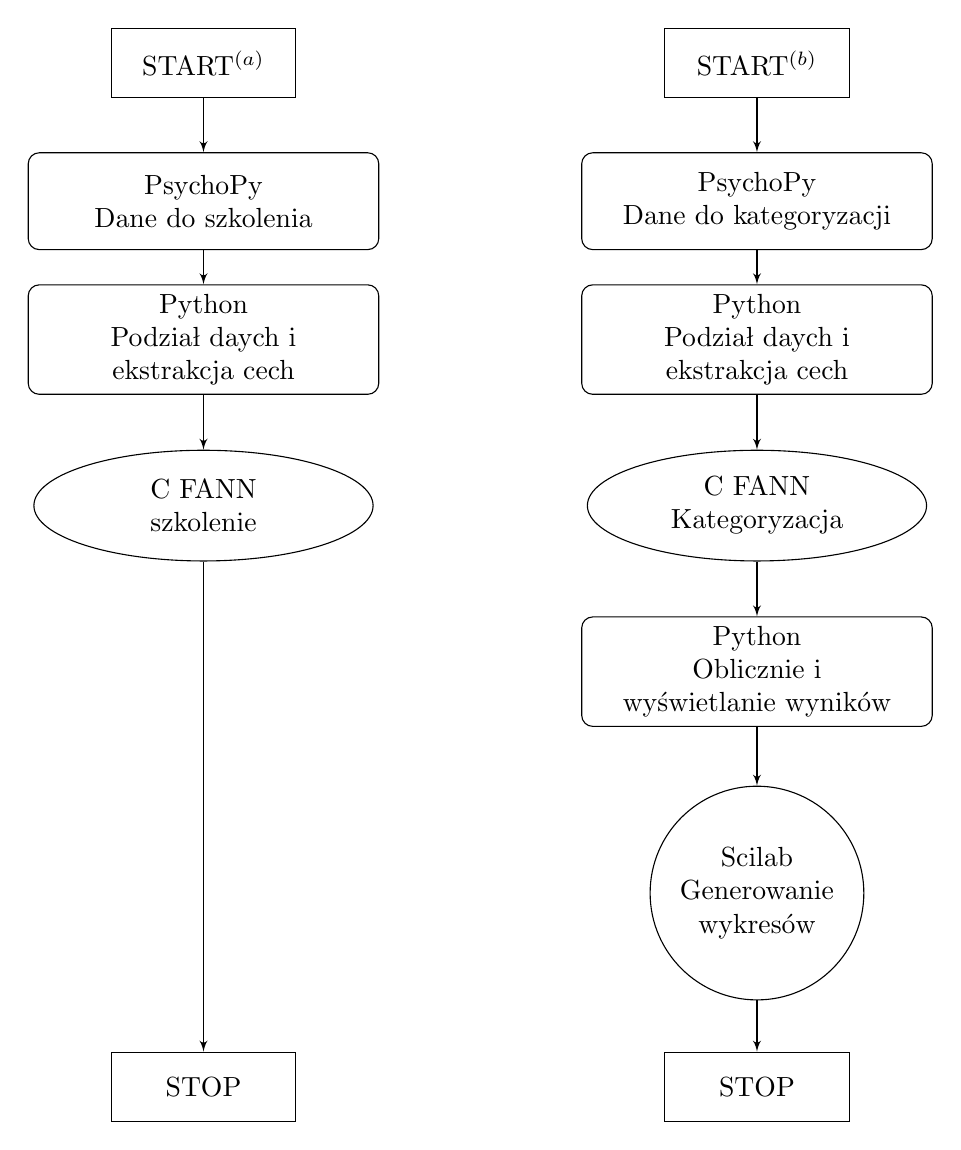
\begin{tikzpicture}[node distance = 2cm, auto]
            % Place nodes
            \node [startstop] (init1) {START$^{(a)}$};
            \node [block, below of=init1, node distance=5em] (psypy1) {PsychoPy \\ Dane do szkolenia};
            \node [block, below of=psypy1, node distance=5em] (extr1) {Python \\Podział daych i ekstrakcja cech};
            \node [cloud, below of=extr1, node distance=6em] (train) {C FANN \\szkolenie};
            \node [startstop, below of=train, node distance=21em] (stop1) {STOP};

            \node [startstop, right of=init1, node distance=20em] (init2) {START$^{(b)}$};
            \node [block, below of=init2, node distance=5em] (psypy2) {PsychoPy \\ Dane do kategoryzacji};
            \node [block, below of=psypy2, node distance=5em] (extr2) {Python \\Podział daych i ekstrakcja cech};
            \node [cloud, below of=extr2, node distance=6em] (categ) {C FANN \\Kategoryzacja};
            \node [block, below of=categ, node distance=6em] (result) {Python \\Oblicznie i wyświetlanie wyników};
            \node [scilab, below of=result, node distance=8em] (sci) {Scilab \\Generowanie wykresów};
            \node [startstop, below of=sci, node distance=7em] (stop2) {STOP};

            % Draw edges
            \path [line] (init1) -- (psypy1);
            \path [line] (psypy1) -- (extr1);
            \path [line] (extr1) -- (train);
            \path [line] (train) -- (stop1);

            \path [line] (init2) -- (psypy2);
            \path [line] (psypy2) -- (extr2);
            \path [line] (extr2) -- (categ);
            \path [line] (categ) -- (result);
            \path [line] (result) -- (sci);
            \path [line] (sci) -- (stop2);

        \end{tikzpicture}
        \hspace*{-2cm} 
        \caption{Schemat zależności między algorytmami w eksperymencie: (a) Etap szkolenia Sieci Neuronalnej, (b) Etap kategoryzacji danych pochodzących od osoby badanej}
    \end{figure}

    Badanie składało się z dwóch etapów: 
    W pierwszym etapie zbierano dane potrzebne do wyszkolenia sieci neuronalnej. Badani mieli za zadanie mrugać gdy zobaczą czerwony kwadrat. Kwadrat ów pojawiał się co 5 sekund na 5 sekund, po czym znikał. Po tym następowało 5 sekund przerwy, w której wyświetlane było jedynie szare tło (bez bodźca). Ten etap trwał 60 sekund. Zatem bodziec wyświetlono 6 razy.
    Drugi etap polegał na kategoryzacji sygnału przez sieć neuronalną. Podczas 60-ciu sekund, które trwało to badanie w losowym momencie (o pełnej sekundzie) pojawiał się bodziec (czerwony kwadrat). W ciągu tej minuty bodziec pojawiał się 14 razy. Było to podyktowane średnią ilością mrugnięć, jakie wykonuje człowiek w ciągu minuty.
    Zadanie osoby badanej w tej części polegało na wykonaniu pojedynczego mrugnięcia gdy zobaczy ona bodziec.
    Minimalna różnica czasowa między eskpozycjami bodźców wynosiła 2 sekundy. Owa założona różnica podyktowana była dwoma czynnikami. Średni interwał między spontanicznymi ludzkimi mrugnięciami wynosi od 2 do 10 sekund. Ponadto przerwa krótsza niż 2 sekundy generuje sporo dodatkowych artefaktów, które utrudniają poprawne skategoryzowanie mrugnięcia oraz odróżnienie jednego mrugnięcia od drugiego. 

    Podczas etapu szkoleniowego dane zapisywane były do dwóch plików w formacie csv: norma\_raw.csv (zawierającego dane z okresu, w których osoba badana nie mrugała) oraz blink\_raw.csv (dane pochodzące z czasu gdy osoba badana mrugała). Za pomocą skryptu w języku programowania Python podzielono dane z obu plików *.csv na paczki po 128 próbek każda (1/4 sekund). Ten sam skrypt ekstraktował cechy ze wspomnianych paczek. Cechy, które ekstraktowane były na potrzeby niniejszego projektu to: odchylenie standardowe sygnału, suma amplitud ujemnych, suma przejść sygnału przez oś OX (0). 
    %Przy doborze cech częściowo inspirowano się artykułem [ŹRÓDŁO].

    Następnie bazując na danych wyekstraktowanych wcześniej stworzono oraz wyszkolono Sztuczną Sieć Neuronalną (ANN). Output z owego szkolenia (dla każdej osoby) dostępny jest w dodatku do sprawozdania. 

    Dane z eksperymentu polegającego na pojedynczych mrugnięciach również podzielono na paczki po 128 próbek. Wykorzystując wcześniej wyszkoloną sieć skategoryzowano każdą paczkę jako mrugnięcie lub nie-mrugnięcie. Jedno mrugnięcie trwa średnio więcej niż 128 próbek (1/4 sekundy). Artefakty w sygnale wywołane mrugnięciem trwają dłużej niż mrugnięcie. Dlatego przyjęto następujące zasady orzekania o poprawności mrugnięcia:
    \newline
    * * *
    \newline
    % Zasady orzekania o poprawności kategoryzacji.
    Założenie wstępne: 
    
    Osoba badana mrugała tylko w przypadku reakcji na bodziec (tak w sesji szkolenia sieci jak i sesji kategoryzacji).
    Egzaminator obserwował osobę badaną. Z badania wyłączono sesje badania, w których badany mrugał w innym przypadku niż pojawienie się bodźca.
    \newline
    * * *

    Uwagi wstępne: 
    Przyjmuje się rozróżnienie pomiędzy czterema obiektami:
    \begin{itemize}
        \item poprawnie skategoryzowana paczka
        \item niepoprawnie skategoryzowana paczka
        \item poprawnie skategoryzowane mrugnięcie
        \item niepoprawnie skategoryzowane mrugnięcie
    \end{itemize}
    Wprowadzenie powyższego rozróżnienia uzasadnione zostanie poniżej.
    \newline
    * * *

    Kategoryzacja mrugnięcia uznana jest za poprawną wtedy i tylko wtedy gdy spełnione są trzy poniższe warunki:
    \begin{enumerate}
        \item Przynajmniej jedna paczka danych, która pokrywa się czasowo z bodźcem została skategoryzowana jako mrugnięcie.
        \item Nie więcej niż 4 paczki (jedna za drugą) z których pierwsza pokrywa się czasowo z bodźcem zostały skategoryzowana jako mrugnięcie.
        \item Jedna lub więcej paczek na przestrzeni czterech kolejnych, z których pierwsza pokrywa się czasowo z bodźcem, zostały skategoryzowana jako mrugnięcie.
    \end{enumerate}
    W każdym innym przypadku skategoryzowanie paczki danych jako mrugnięcie uważane jest za niepoprawne.
    \newline
    * *
   
    Wszystkie paczki skategoryzowane jako niepoprawne grupuje się w następujący sposób jako niepoprawnie skategoryzowane mrugnięcie:
    \begin{enumerate}
        \item Jeżeli jakakolwiek z paczek została niepoprawnie skategoryzowana, to zarówno ją jak i trzy następujące po niej paczki niepoprawnie skategoryzowane (jeśli takowe występują) uważa się za niepoprawnie skategoryzowane mrugnięcie.
        \item Do dalszego rozpoznawania ciągu paczek jako nie-mrugnięć nie bierze się pod uwagę ciągów wcześniej skategoryzowanych jako nie-mrugnięcie (ani ich poszczególnych elementów).
    \end{enumerate}
    * * *
    
    W nawiązaniu do powyższego proponujemy ustalenie trzech wskaźników (dotyczących etapu kategoryzacji) poprawności algorytmów:
    \begin{enumerate}
        \item Wskaźnik\_01. Jest to wskaźnik poprawności kategoryzacji mrugnięcia jako odpowiedzi na bodziec.
    Jest to stosunek poprawnie skategoryzowanych mrugnięć do ilości bodźców zaprezentowanych w danym eksperymencie.
    Stosunek ten wyrażono w procentach.
        \item Wskaźnik\_02. Jest to wskaźnik braku poprawności mrugnięcia w odniesieniu do ilości bodźców w eksperymencie.
    Jest to stosunek ilości błędnie skategoryzowanych mrugnięć do ilości bodźców w eksperymencie.
    Stosunek ten wyrażono w procentach.
        \item Wskaźnik\_03. Jest to wskaźnik braku poprawności mrugnięcia w odniesieniu do ilości poprawnie skategoryzowanych mrugnięć.
    Jest to stosunek ilości błędnie skategoryzowanych mrugnięć do ilości poprawnie skategoryzowanych mrugnięć. 
    Stosunek ten wyrażono w procentach.
    \end{enumerate}
    Etap kategoryzacji dla każdej osoby był oceniany ze względu na trzy powyższe wskaźniki. %~\cite{Abootalebia2009}
    \vspace{\baselineskip}

    Jako wynik ogólny kategoryzacji rozumie się rożnicę Wskaźnika\_01 oraz Wskaźnika\_02.
    \vspace{\baselineskip}

    Jako wartość wskaźnika dla wszystkich osób rozumie się średnią wyników wskaźnika dla poszczególnych osób.
    \vspace{\baselineskip}

    Wskaźnik\_03 jest wskaźnikiem pomocniczym i nie jest brany pod uwagę przy ustalaniu wyniku ogólnego kategoryzacji.

    \subsection{Opis zbioru danych}
    Częstotliwość próbkowania MindWave Mobile wynosi 512 Hz. Czyli EEG podaje wartość napięcia (w mikro Voltach) 512 razy na sekundę. Pojedynczy odczyt nazywany będzie w dalszej części pracy próbką (samplem). Natomiast zbiór próbek będzie nosił miano paczki (paczki danych).
    Przykładowe 10 kolejnych próbek zostało przedstawione w tabeli poniżej.
    \newline
    \begin{table}[h]
        \begin{center}
        \caption[Table caption text]{Sygnał MindWave Mobile EEG z jednej elektrody czołowej.\\ Przykładowe 10 kolejnych próbek.}
%         \csvautotabular{../csv_eeg_ann/mwm_10_samples_eeg_01.csv}
        \csvautotabular{mwm_10_samples_eeg_01.csv}
        \end{center}
    \end{table}
 % % %

%%%%%%%%%%%%%%%%%%%%%%%%%%%%%%%%%%%%%%%%%%%%%%%%%%%%%%%%%%%%%%%%
%    RESULTS    RESULTS    RESULTS                             %
%%%%%%%%%%%%%%%%%%%%%%%%%%%%%%%%%%%%%%%%%%%%%%%%%%%%%%%%%%%%%%%%
\newpage
\section{Wyniki}
    \subsection{Wartości wskaźników}

    W poniższej tabeli zaprezentowano wyniki wskaźników dla trzech osób badanych. \\

    \begin{table}[H]
        \caption {Wartości wkaźników dla poszczególnych osób badanych}
        \begin{center}
            \begin{tabular}{| p{2.75cm} || c | c | c | c |}
                \hline
                 & Osoba 001 & Osoba 002 & Osoba 003 & Wszystkie osoby \\
                \hline
                \hline
                Wskaźnik\_01 & 100\% & 100\% & 100\% & 100\% \\
                \hline
                Wskaźnik\_02 &   0\% &  71\% &  28\% &  33\% \\
                \hline
                Wskaźnik\_03 &   0\% &  71\% &  28\% &  33\% \\
                \hline
                \hline
                Ogólny wynik & 100\% &  29\% &  72\% &  67\% \\
                \hline
            \end{tabular}
        \end{center}
    \end{table}

    Objaśnienia do tabeli "Wartości wskaźników dla poszczególnych osób badanych":
    \begin{itemize}
        \item Osoba 001, ..., Osoba n - kolumny pokazujące wskaźniki dla poszczególnych osób badanych
        \item Wskaźnik\_01, Wskaźnik\_02 oraz Wskaźnik\_03 - wskaźniki opisane w sekcji pt. "Materiały i metody"
        \item Wszystkie osoby - średni wynik wskaźnika dla wszystkich osób badanych
        \item Ogólny wynik - różnica Wskaźnika pierwszego oraz Wskaźnika drugiego - według wytycznych z sekcji pt. "Materiały i metody"
    \end{itemize}



    Wykresy oraz wyniki kategoryzacji dla poszczególnych osób dostępne są w dodatku do tego sprawozdania.

    \newpage
    \subsection{Przykład tabeli z mrugnięciami oraz wykresów \\Osoba 003}
        Objaśnienia do tabeli dotyczących paczek oraz grupowania ich w mrugnięcia:\
        \begin{itemize}
            \item Nr paczki - numer paczki, która została skategoryzowana jako mrugnięcie.
            \item Względem bodźca - czy zasięg paczki pokrywa się z zasięgiem występowania bodźca czy nie. 
            \begin{itemize}
                \item[*] 0 - nie pokrywa się\
                \item[*] 1 - pokrywa się\
            \end{itemize}
            \item Numer mrugnięcia - grupowanie paczek w mrugnięcia na podstawie wcześniejszych założeń. Do tabeli ze wszystkimi paczkami razem: jeśli mrugnięcie ma numer 0 znaczy to, że paczka ta jest niepoprawnie skategoryzowana. W kolejnych tabelach mrugnięcia są rodzielane na poprawnie oraz niepoprawnie skategoryzowane.
            \item Początek paczki - numer próbki, na której zaczyna się paczka skategoryzowana jako mrugnięcie.
            \item Koniec paczki - numer próbki, na której kończy się paczka skategoryzowana jako mrugnięcie. 
        \end{itemize}


        \begin{table}[H]
            \captionsetup{justification=centering}
            \caption {Wszystkie paczki skategoryzowane jako mrugnięcia. \\ Osoba 003}
            \begin{center}
                \begin{tabular}{| p{1cm} | p{1.75cm} | p{1.75cm} | p{1.75cm} | p{1.75cm} |}
                    \hline
                    Nr paczki & Względem bodźca & Numer mrugnięcia & Początek paczki & Koniec paczki \\
                    \hline
                    \hline
                    01 & 1 & 1 & 1024 & 1150 \\
                    \hline
                    02 & 1 & 1 & 1152 & 1278 \\
                    \hline
                    03 & 0 & 1 & 1280 & 1406 \\
                    \hline
                    04 & 0 & 0 & 2048 & 2174 \\
                    \hline
                    05 & 1 & 2 & 2560 & 2686 \\
                    \hline
                    06 & 1 & 2 & 2688 & 2814 \\
                    \hline
                    07 & 0 & 2 & 2816 & 2942 \\
                    \hline
                    08 & 1 & 3 & 4224 & 4350 \\
                    \hline
                    09 & 0 & 3 & 4352 & 4478 \\
                    \hline
                    10 & 0 & 0 & 4864 & 4990 \\
                    \hline
                    11 & 1 & 4 & 6656 & 6782 \\
                    \hline
                    12 & 1 & 4 & 6784 & 6910 \\
                    \hline
                    13 & 0 & 4 & 6912 & 7038 \\
                    \hline
                    14 & 1 & 5 & 9344 & 9470 \\
                    \hline
                    15 & 0 & 5 & 9472 & 9598 \\
                    \hline
                    16 & 1 & 6 & 10880 & 11006 \\
                    \hline
                    17 & 1 & 7 & 12416 & 12542 \\
                    \hline
                    18 & 1 & 8 & 13952 & 14078 \\
                    \hline
                    19 & 1 & 8 & 14080 & 14206 \\
                    \hline
                    20 & 1 & 9 & 16000 & 16126 \\
                    \hline
                    21 & 1 & 9 & 16128 & 16254 \\
                    \hline
                    22 & 1 & 10 & 17536 & 17662 \\
                    \hline
                    23 & 1 & 10 & 17664 & 17790 \\
                    \hline
                    24 & 1 & 11 & 19584 & 19710 \\
                    \hline
                    25 & 1 & 11 & 19712 & 19838 \\
                    \hline
                    26 & 0 & 0 & 21376 & 21502 \\
                    \hline
                    27 & 1 & 12 & 23168 & 23294 \\
                    \hline
                    28 & 1 & 12 & 23296 & 23422 \\
                    \hline
                    29 & 1 & 13 & 25728 & 25854 \\
                    \hline
                    30 & 1 & 13 & 25856 & 25982 \\
                    \hline
                    31 & 1 & 14 & 27264 & 27390 \\
                    \hline
                    32 & 1 & 14 & 27392 & 27518 \\
                    \hline
                    33 & 0 & 0 & 27520 & 27646 \\
                    \hline
                \end{tabular}
            \end{center}
        \end{table}

        \begin{table}[H]
            \captionsetup{justification=centering}
            \caption {Zbiory paczek poprawnie skategoryzowanych jako mrugnięcia. \\ Osoba 003}
            \begin{center}
                \begin{tabular}{| p{1cm} | p{1.75cm} | p{1.75cm} | p{1.75cm} | p{1.75cm} |}
                    \hline
                    Nr paczki & Względem bodźca & Numer mrugnięcia & Początek paczki & Koniec paczki \\
                    \hline
                    \hline
                    01 & 1 & 1 & 1024 & 1150 \\
                    \hline
                    02 & 1 & 1 & 1152 & 1278 \\
                    \hline
                    03 & 0 & 1 & 1280 & 1406 \\
                    \hline
                    04 & 1 & 2 & 2560 & 2686 \\
                    \hline
                    05 & 1 & 2 & 2688 & 2814 \\
                    \hline
                    06 & 0 & 2 & 2816 & 2942 \\
                    \hline
                    07 & 1 & 3 & 4224 & 4350 \\
                    \hline
                    08 & 0 & 3 & 4352 & 4478 \\
                    \hline
                    09 & 1 & 4 & 6656 & 6782 \\
                    \hline
                    10 & 1 & 4 & 6784 & 6910 \\
                    \hline
                    11 & 0 & 4 & 6912 & 7038 \\
                    \hline
                    12 & 1 & 5 & 9344 & 9470 \\
                    \hline
                    13 & 0 & 5 & 9472 & 9598 \\
                    \hline
                    14 & 1 & 6 & 10880 & 11006 \\
                    \hline
                    15 & 1 & 7 & 12416 & 12542 \\
                    \hline
                    16 & 1 & 8 & 13952 & 14078 \\
                    \hline
                    17 & 1 & 8 & 14080 & 14206 \\
                    \hline
                    18 & 1 & 9 & 16000 & 16126 \\
                    \hline
                    19 & 1 & 9 & 16128 & 16254 \\
                    \hline
                    20 & 1 & 10 & 17536 & 17662 \\
                    \hline
                    21 & 1 & 10 & 17664 & 17790 \\
                    \hline
                    22 & 1 & 11 & 19584 & 19710 \\
                    \hline
                    23 & 1 & 11 & 19712 & 19838 \\
                    \hline
                    24 & 1 & 12 & 23168 & 23294 \\
                    \hline
                    25 & 1 & 12 & 23296 & 23422 \\
                    \hline
                    26 & 1 & 13 & 25728 & 25854 \\
                    \hline
                    27 & 1 & 13 & 25856 & 25982 \\
                    \hline
                    28 & 1 & 14 & 27264 & 27390 \\
                    \hline
                    29 & 1 & 14 & 27392 & 27518 \\
                    \hline
                \end{tabular}
            \end{center}
        \end{table}

        \begin{table}[H]
            \captionsetup{justification=centering}
            \caption {Zbiory paczek niepoprawnie skategoryzowanych jako mrugnięcia. \\Osoba 003}
            \begin{center}
                \begin{tabular}{| p{1cm} | p{1.75cm} | p{1.75cm} | p{1.75cm} | p{1.75cm} |}
                    \hline
                    Nr paczki & Względem bodźca & Numer mrugnięcia & Początek paczki & Koniec paczki \\
                    \hline
                    \hline
                    01 & 0 & 1 & 2048 & 2174 \\
                    \hline
                    02 & 0 & 2 & 4864 & 4990 \\
                    \hline
                    03 & 0 & 3 & 21376 & 21502 \\
                    \hline
                    04 & 0 & 4 & 27520 & 27646 \\
                    \hline
                \end{tabular}
            \end{center}
        \end{table}

        \subsection{Przykładowe wykresy danych osoby badanej \\Osoba 003}

            Poniżej zaprezentowano przykładowy wykres dla osoby badanej 003.
            \newline
            Wszystkie wykresy wraz z dokładnymi danymi znajdują się w dodatku załączonym na końcu sprawozdania.
            
            \begin{figure}[H]
                \hspace*{-4.5cm} 
                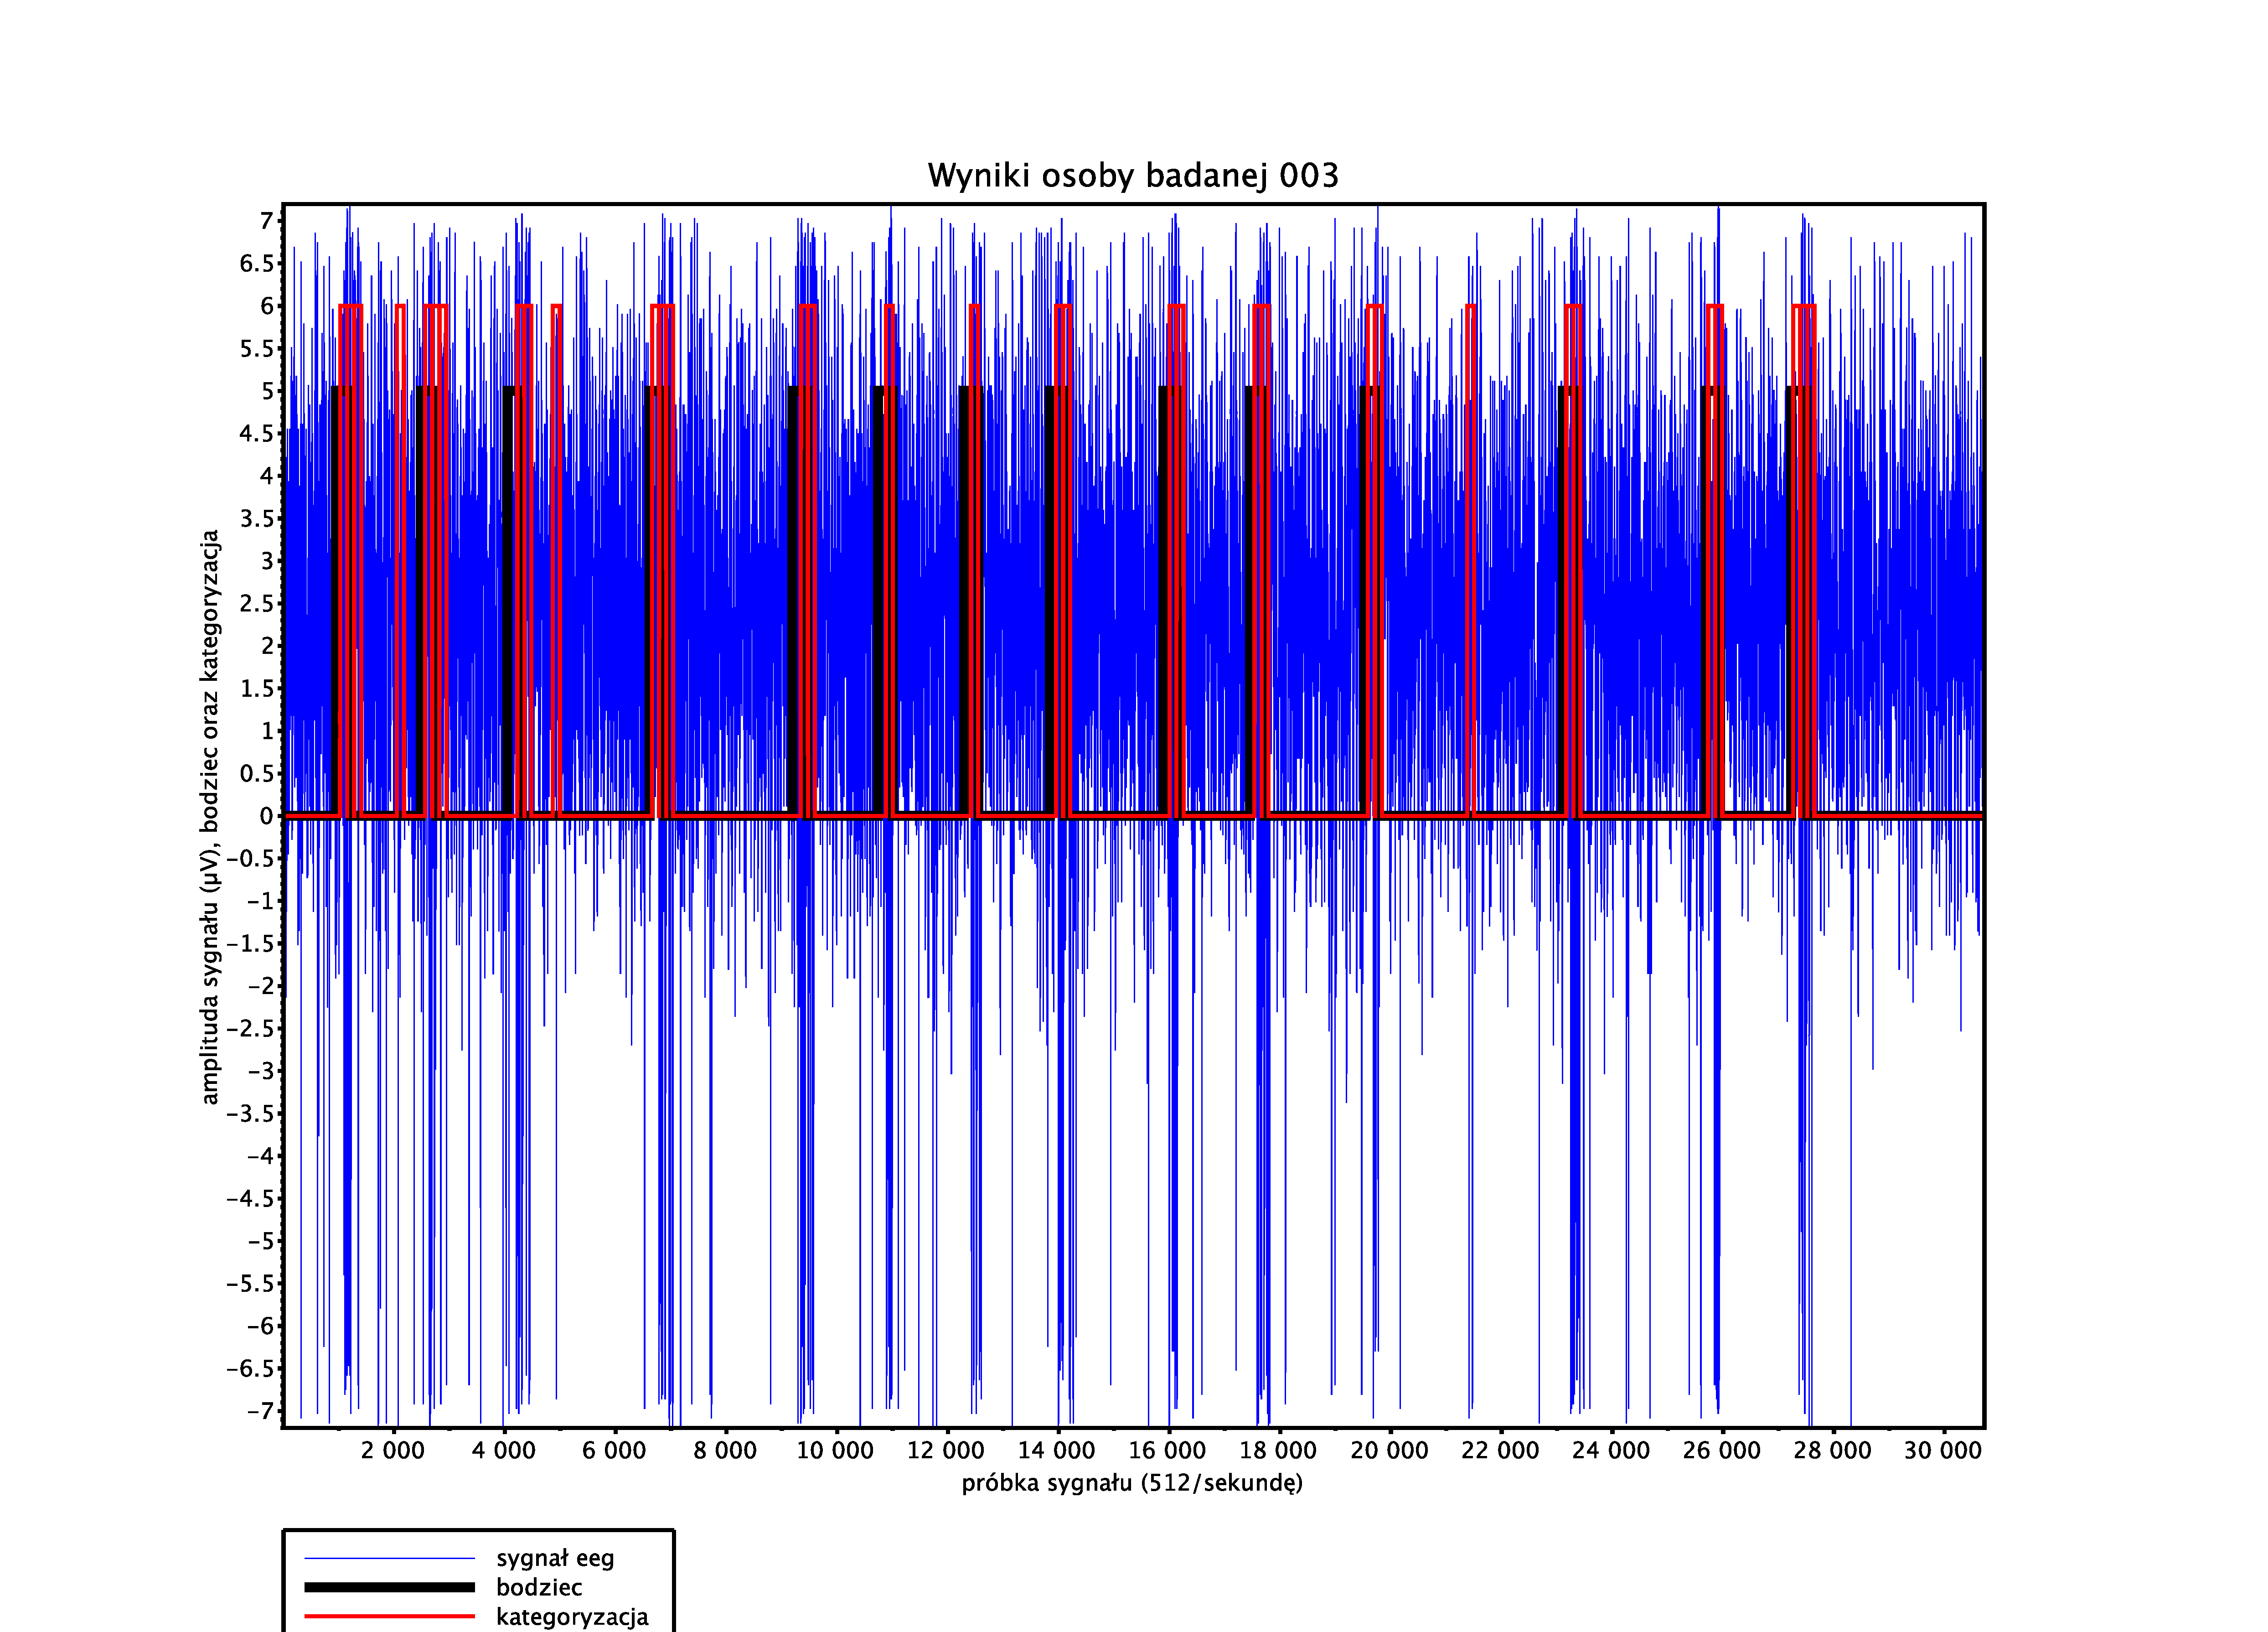
\includegraphics[width=\linewidth+10cm]{../plotting_data/scilab_eeg_01_sub_003.pdf}
                \caption{Dane dla osoby badanej 003}
            \end{figure}
            


        %


    % % %

    %%%%%%%%%%%%%%%%%%%%%%%%%%%%%%%%%%%%%%%%%%%%%%%%%%%%%%%%%%%%%%%%
    %    DISCUSSION    DISCUSSION    DISCUSSION                    %
    %%%%%%%%%%%%%%%%%%%%%%%%%%%%%%%%%%%%%%%%%%%%%%%%%%%%%%%%%%%%%%%%
    \newpage
    \section{Dyskusja}
        Metody uczenia maszynowego algorytmów są coraz częściej wykorzystywane w różnych dziedzinach nauki oraz życia. Wyniki uzyskane w przedstawionym eksperymencie potwierdzają zasadność używania takiego podejścia także do interpretowania danych pochodzących z EEG. 
        
        Całe badanie, wraz ze szkoleniem sieci neuronalnych trwa około trzech minut. Można skrócić ten czas w pełni automatyzując procesy uruchamiania eksperymentów oraz szkolenia sieci (szkolenie owo miałoby się odbywać podczas czytania instrukcji i wykonywania drugiej części eksperymentu). Już teraz, w ciągu owych trzech minut, algorytm jest w stanie skategoryzować mrugnięcie na poziomie XYZ \%. Gdyby wprowadzić pewne poprawki (patrz poniżej) lub przedłużyć czas trwania szkolenia o kolejne sesje treningowe dla sieci (również poniżej) możnaby osiągnąć wyniki rzędu 90-100 \% poprawnych kategoryzacji.

        Bardzo ważne jest by osoba badana podczas etapu szkolenia sieci neuronalnych nie wykonywała żadnych ruchów poza ruchami mięśni powiek. Ten czynnik jest krytyczny jeśli chodzi o szkolenie (tutaj liczy się także częstotliwość mrugania) oraz rozpoznawanie pojedynczych mrugnięć. Proponuje się załączenie filmu instruktażowego do instrukcji wykonywania etapu szkolenia. Na filmie pokreślonoby ruchy jedynie mięśni powiek oraz pokazywałoby poprawną częstotliwość owych ruchów.

        Niski wynik dla osoby badanej 002 wynika z trzech czynników. Czynniki te, jako mogące wpływać negatywnie na wyniki szkolenia oraz kategoryzacji, zostaną poniżej pokrótce opisane. Zaproponowano też rozwiązania pozwalające zniwelować lub zmniejszyć wpływ owych czynników na wyniki badania.
            \begin{enumerate}
                \item Słabe przeszkolenie osoby badanej. Osoba prawdopodobnie wynonywała ruchy mięśniami powiek lub twarzy także poza pojawieniem się bodźca. \\
                    Rozwiązania: 
                    \begin{itemize}
                        \item Dołącznie filmu instruktarzowego do instrukcji przed rozpoczęciem badania. 
                        \item Zebranie większej ilości materiału i wyłączenie z sesji szkolenia sieci danych niebędących mruganiem. 
                    \end{itemize}
                \item Sieć neuronalna była przeuczona. Zbytnia czułość kategoryzacji brała artefakty o innym źródle niż mruganie za mrugnięcie.
                    Rozwiązania: patrz: Proponowane rozwiązania algorytmiczne mające na celu zwiększenie poprawności kategoryzacji mrugnięć przez ANN.
                \item Możliwe są błędy algorytmiczne przy zbieraniu danych.\\
                    Autorzy skorzystali z gotowego skryptu w języku programowania Python na pobieranie danych z urządzenia MindWave Moblie. Przez specyfikę urządzenia zdarza się, że sporadycznie gubi ono paczki z danymi zawiarającymi informację o sygnale. Podejrzewa się, że przy owym gubieniu paczek dochodzi do kontaminacji informacji przez nadmiarowe lub nieodpowiednie dane (niemające związku z sygnałem z samego EEG). Warte podkreślenia jest tutaj, że pomimo owych "zakłóceń" sieć neurnonalna, szkolona na tak małym i niepewnym materiale, jest w stanie w miarę poprawnie skategoryzować mrugnięcie. \\
                    Rozwiązania: 
                    \begin{itemize}
                        \item Zmiana systemu operacyjnego oraz języka programowania używanego do komunikacji z MindWave Mobile. 
                        \item Znalezienie źródła problemu w programie w języku Python lub upewnienie się, że to kwestia samego skryptu, a nie platformy, na której wykonywano badanie (Linux) lub sprzętu Bluetooth w komputerze, na którym przeprowadzano badanie.
                    \end{itemize}
            \end{enumerate}

        \subsection{Proponowane rozwiązania algorytmiczne mające na celu zwiększenie poprawności kategoryzacji mrugnięć przez ANN}
            Aby zwiększyć poprawność rozpoznawania mrugnięcia proponuje się następujące rozwinięcia algorytmiczne:
            \begin{enumerate}
                \item Zastosowanie rozwiązań ewolucyjnych przy doborze cech ekstraktowanych z surowego sygnału (algorytmy genetyczne). Cechy ekstraktwowane z sygnału w niniejszym sprawozdaniu mogą nie być optymalne do późniejszego szkolenia oraz kategoryzacji paczek jako mrugnięcia lub nie-mrugnięcia.
                \item Wdrożenie podejścia Bayesowskiego przy poprawnej lub niepoprawnej kategoryzacji paczki jako mrugnięcie. Należy budować kolejne bazy danych do szkolenia sieci neuronalnych na podstawie kategoryzacji paczek jako mrugnięć lub nie-mrugnięć w etapie kategoryzacji bodźców. Na nowo ustruktyryzowanych danych należy wyszkolić po raz kolejny sieć neuronalną i to na niej oprzeć późniejszą kategoryzację.
%                     [tutaj być może obrazek z wykresem ułatwiający zrozumienie tematu]
            \end{enumerate}



    % % %

    \newpage
    \begin{thebibliography}{50}
        \bibitem{} Augustyniak P., \emph{Przetwarzanie sygnałów elektrodiagnostycznych}, AGH Uczelniane Wydawnictwa Naukowo-Dydaktyczne, 2001.
        \bibitem{} Abootalebi V., Moradi M. H., Khalilzadeh M. A., \emph{A new approach for EEG feature extraction in P300-based lie detection}, Computer Methods and Programs in Biomedicine 94 (2009) 48-57
        \bibitem{} Chambayil B., Singla R., Jha R., \emph{EEG Eye Blink Classification Using Neural Network}, Proceedings of the World Congress on Engineering 2010 Vol I, WCE 2010, June 30 - July 2, 2010, London, U.K.
        \bibitem{} http://www.reviewofophthalmology.com/content/d/therapeutic\_topics/i/1290/c/24850/
    \end{thebibliography}
    % % %

    \newpage
    \section*{Dodatek A: Programy oraz skrypty}
        \subsection*{Eksperyment w PsychoPy zbierający dane do szkolenia ANN}
        \subsection*{Skrypt C FANN tworzący oraz szkolący \\Sztuczną Sieć Neuronalną}
        \subsection{Eksperyment w PsychoPy zbierający dane \\do późniejszej kategoryzacji przez ANN}
        \subsection{Skrypt C FANN kategoryzujący poszczególne paczki danych \\jako mrugnięcie lub nie-mrugnięcie}
        \subsection{Skrypt Python generujący pliki z wynikami}
        \subsection{Skrypt Scilab generujący wykresy}
    % % %

    \newpage
    \section*{Dodatek B: Szczegółowe wyniki}

        Objaśnienia do tabeli dotyczących paczek oraz grupowania ich w mrugnięcia: 
        \begin{itemize}
            \item Nr paczki - numer paczki, która została skategoryzowana jako mrugnięcie.
            \item Względem bodźca - czy zasięg paczki pokrywa się z zasięgiem występowania bodźca czy nie. 
            \begin{itemize}
                \item[*] 0 - nie pokrywa się\
                \item[*] 1 - pokrywa się\
            \end{itemize}
            \item Numer mrugnięcia - grupowanie paczek w mrugnięcia na podstawie wcześniejszych założeń.
            \item Początek paczki - numer próbki, na której zaczyna się paczka skategoryzowana jako mrugnięcie.
            \item Koniec paczki - numer próbki, na której kończy się paczka skategoryzowana jako mrugnięcie. 
        \end{itemize}

        Zamieszczone zostały tutaj tabele z mrugnięciami już podzielonymi na paczki poprawnie oraz niepoprawnie skaregoryzowane. Pogrupowane też zostały owe paczki w poprawnie skategoryzowane mrugnięcia oraz niepoprawnie skategoryzowane mrugnięcia.

        \subsection*{Osoba pierwsza}
            \begin{table}[H]
                \captionsetup{justification=centering}
                \caption {Zbiory paczek poprawnie skategoryzowanych jako mrugnięcia. \\ Osoba 001}
                \begin{center}
                    \begin{tabular}{| p{1cm} | p{1.75cm} | p{1.75cm} | p{1.75cm} | p{1.75cm} |}
                        \hline
                        Nr paczki & Względem bodźca & Numer mrugnięcia & Początek paczki & Koniec paczki \\
                        \hline
                        \hline
                        01 & 1 & 1 & 1152 & 1278 \\ 
                        \hline
                        02 & 1 & 1 & 1280 & 1406 \\ 
                        \hline
                        03 & 0 & 1 & 1408 & 1534 \\ 
                        \hline
                        04 & 1 & 2 & 2816 & 2942 \\ 
                        \hline
                        05 & 0 & 2 & 2944 & 3070 \\ 
                        \hline
                        06 & 0 & 2 & 3072 & 3198 \\ 
                        \hline
                        07 & 1 & 3 & 4608 & 4734 \\ 
                        \hline
                        08 & 1 & 3 & 4864 & 4990 \\ 
                        \hline
                        09 & 0 & 3 & 4992 & 5118 \\ 
                        \hline
                        10 & 1 & 4 & 6400 & 6526 \\ 
                        \hline
                        11 & 1 & 5 & 10496 & 10622 \\ 
                        \hline
                        12 & 0 & 5 & 10624 & 10750 \\ 
                        \hline
                        13 & 1 & 6 & 12032 & 12158 \\ 
                        \hline
                        14 & 1 & 6 & 12160 & 12286 \\ 
                        \hline
                        15 & 1 & 7 & 15616 & 15742 \\ 
                        \hline
                        16 & 1 & 7 & 15744 & 15870 \\ 
                        \hline
                        17 & 1 & 8 & 17152 & 17278 \\ 
                        \hline
                        18 & 1 & 8 & 17280 & 17406 \\ 
                        \hline
                        19 & 1 & 9 & 18688 & 18814 \\ 
                        \hline
                        20 & 1 & 9 & 18816 & 18942 \\ 
                        \hline
                        21 & 1 & 10 & 20224 & 20350 \\ 
                        \hline
                        22 & 1 & 10 & 20352 & 20478 \\ 
                        \hline
                        23 & 1 & 11 & 21888 & 22014 \\ 
                        \hline
                        24 & 1 & 12 & 24448 & 24574 \\ 
                        \hline
                        25 & 0 & 12 & 24576 & 24702 \\ 
                        \hline
                        26 & 1 & 13 & 26496 & 26622 \\ 
                        \hline
                        27 & 0 & 13 & 26624 & 26750 \\ 
                        \hline
                        28 & 1 & 14 & 28032 & 28158 \\ 
                        \hline
                        29 & 0 & 14 & 28544 & 28670 \\ 
                        \hline
                    \end{tabular}
                \end{center}
            \end{table}

            \begin{table}[H]
                \captionsetup{justification=centering}
                \caption {Zbiory paczek niepoprawnie skategoryzowanych jako mrugnięcia. \\Osoba 001}
                \begin{center}
                    \begin{tabular}{| p{1cm} | p{1.75cm} | p{1.75cm} | p{1.75cm} | p{1.75cm} |}
                        \hline
                        Nr paczki & Względem bodźca & Numer mrugnięcia & Początek paczki & Koniec paczki \\
                        \hline
                        \hline
                        brak & brak & brak & brak & brak \\ 
                        \hline
                    \end{tabular}
                \end{center}
            \end{table}

            Zgodnie z wcześniej przyjętymi kryteriami dla osoby badanej 001 nie ma niepoprawnie skategoryzowanych mrugnięć.

        \newpage
        \subsection*{Osoba druga}
            \begin{table}[H]
                \captionsetup{justification=centering}
                \caption {Zbiory paczek poprawnie skategoryzowanych jako mrugnięcia. \\ Osoba 002}
                \begin{center}
                    \begin{tabular}{| p{1cm} | p{1.75cm} | p{1.75cm} | p{1.75cm} | p{1.75cm} |}
                        \hline
                        Nr paczki & Względem bodźca & Numer mrugnięcia & Początek paczki & Koniec paczki \\
                        \hline
                        \hline
                        01 & 1 & 1 & 1408 & 1534  \\
                        \hline
                        01 & 1 & 1 & 1408 & 1534  \\
                        \hline
                        02 & 1 & 1 & 1536 & 1662  \\
                        \hline
                        03 & 0 & 1 & 1664 & 1790  \\
                        \hline
                        04 & 1 & 2 & 2944 & 3070  \\
                        \hline
                        05 & 1 & 2 & 3072 & 3198  \\
                        \hline
                        06 & 1 & 2 & 3200 & 3326  \\
                        \hline
                        07 & 1 & 3 & 5120 & 5246  \\
                        \hline
                        08 & 1 & 3 & 5248 & 5374  \\
                        \hline
                        09 & 1 & 4 & 6656 & 6782  \\
                        \hline
                        10 & 1 & 4 & 6784 & 6910  \\
                        \hline
                        11 & 0 & 4 & 6912 & 7038  \\
                        \hline
                        12 & 1 & 5 & 9728 & 9854  \\
                        \hline
                        13 & 1 & 5 & 9856 & 9982  \\
                        \hline
                        14 & 1 & 6 & 11264 & 11390  \\
                        \hline
                        15 & 1 & 6 & 11392 & 11518  \\
                        \hline
                        16 & 0 & 6 & 11520 & 11646  \\
                        \hline
                        17 & 1 & 7 & 13824 & 13950  \\
                        \hline
                        18 & 1 & 7 & 13952 & 14078  \\
                        \hline
                        19 & 0 & 7 & 14080 & 14206  \\
                        \hline
                        20 & 1 & 8 & 16384 & 16510  \\
                        \hline
                        21 & 1 & 8 & 16512 & 16638  \\
                        \hline
                        22 & 0 & 8 & 16640 & 16766  \\
                        \hline
                        23 & 1 & 9 & 17920 & 18046  \\
                        \hline
                        24 & 1 & 9 & 18048 & 18174  \\
                        \hline
                        25 & 0 & 9 & 18176 & 18302  \\
                        \hline
                        26 & 1 & 10 & 22144 & 22270  \\
                        \hline
                        27 & 0 & 10 & 22272 & 22398  \\
                        \hline
                        28 & 1 & 11 & 23552 & 23678  \\
                        \hline
                        29 & 1 & 11 & 23680 & 23806  \\
                        \hline
                        30 & 0 & 11 & 23808 & 23934  \\
                        \hline
                        31 & 1 & 12 & 25216 & 25342  \\
                        \hline
                        32 & 1 & 13 & 26752 & 26878  \\
                        \hline
                        33 & 1 & 13 & 26880 & 27006  \\
                        \hline
                        34 & 0 & 13 & 27008 & 27134  \\
                        \hline
                        35 & 1 & 14 & 28288 & 28414  \\
                        \hline
                    \end{tabular}
                \end{center}
            \end{table}

            \begin{table}[H]
                \captionsetup{justification=centering}
                \caption {Zbiory paczek niepoprawnie skategoryzowanych jako mrugnięcia. \\Osoba 002}
                \begin{center}
                    \begin{tabular}{| p{1cm} | p{1.75cm} | p{1.75cm} | p{1.75cm} | p{1.75cm} |}
                        \hline
                        Nr paczki & Względem bodźca & Numer mrugnięcia & Początek paczki & Koniec paczki \\
                        \hline
                        \hline
                        01 & 0 & 1 & 128 & 254 \\
                        \hline
                        02 & 0 & 2 & 2688 & 2814 \\
                        \hline
                        03 & 0 & 3 & 6400 & 6526 \\
                        \hline
                        04 & 0 & 4 & 7168 & 7294 \\
                        \hline
                        05 & 0 & 5 & 8576 & 8702 \\
                        \hline
                        06 & 0 & 6 & 10240 & 10366 \\
                        \hline
                        07 & 0 & 7 & 13056 & 13182 \\
                        \hline
                        08 & 0 & 7 & 13312 & 13438 \\
                        \hline
                        09 & 0 & 8 & 13568 & 13694 \\
                        \hline
                        10 & 0 & 9 & 17024 & 17150 \\
                        \hline
                        11 & 0 & 10 & 24192 & 24318 \\
                        \hline
                        12 & 0 & 10 & 24320 & 24446 \\
                        \hline
                    \end{tabular}
                \end{center}
            \end{table}

        \subsection*{Osoba trzecia}
            \begin{table}[H]
                \captionsetup{justification=centering}
                \caption {Zbiory paczek poprawnie skategoryzowanych jako mrugnięcia. \\ Osoba 003}
                \begin{center}
                    \begin{tabular}{| p{1cm} | p{1.75cm} | p{1.75cm} | p{1.75cm} | p{1.75cm} |}
                        \hline
                        Nr paczki & Względem bodźca & Numer mrugnięcia & Początek paczki & Koniec paczki \\
                        \hline
                        \hline
                        01 & 1 & 1 & 1024 & 1150 \\
                        \hline
                        02 & 1 & 1 & 1152 & 1278 \\
                        \hline
                        03 & 0 & 1 & 1280 & 1406 \\
                        \hline
                        04 & 1 & 2 & 2560 & 2686 \\
                        \hline
                        05 & 1 & 2 & 2688 & 2814 \\
                        \hline
                        06 & 0 & 2 & 2816 & 2942 \\
                        \hline
                        07 & 1 & 3 & 4224 & 4350 \\
                        \hline
                        08 & 0 & 3 & 4352 & 4478 \\
                        \hline
                        09 & 1 & 4 & 6656 & 6782 \\
                        \hline
                        10 & 1 & 4 & 6784 & 6910 \\
                        \hline
                        11 & 0 & 4 & 6912 & 7038 \\
                        \hline
                        12 & 1 & 5 & 9344 & 9470 \\
                        \hline
                        13 & 0 & 5 & 9472 & 9598 \\
                        \hline
                        14 & 1 & 6 & 10880 & 11006 \\
                        \hline
                        15 & 1 & 7 & 12416 & 12542 \\
                        \hline
                        16 & 1 & 8 & 13952 & 14078 \\
                        \hline
                        17 & 1 & 8 & 14080 & 14206 \\
                        \hline
                        18 & 1 & 9 & 16000 & 16126 \\
                        \hline
                        19 & 1 & 9 & 16128 & 16254 \\
                        \hline
                        20 & 1 & 10 & 17536 & 17662 \\
                        \hline
                        21 & 1 & 10 & 17664 & 17790 \\
                        \hline
                        22 & 1 & 11 & 19584 & 19710 \\
                        \hline
                        23 & 1 & 11 & 19712 & 19838 \\
                        \hline
                        24 & 1 & 12 & 23168 & 23294 \\
                        \hline
                        25 & 1 & 12 & 23296 & 23422 \\
                        \hline
                        26 & 1 & 13 & 25728 & 25854 \\
                        \hline
                        27 & 1 & 13 & 25856 & 25982 \\
                        \hline
                        28 & 1 & 14 & 27264 & 27390 \\
                        \hline
                        29 & 1 & 14 & 27392 & 27518 \\
                        \hline
                    \end{tabular}
                \end{center}
            \end{table}

            \begin{table}[H]
                \captionsetup{justification=centering}
                \caption {Zbiory paczek niepoprawnie skategoryzowanych jako mrugnięcia. \\Osoba 003}
                \begin{center}
                    \begin{tabular}{| p{1cm} | p{1.75cm} | p{1.75cm} | p{1.75cm} | p{1.75cm} |}
                        \hline
                        Nr paczki & Względem bodźca & Numer mrugnięcia & Początek paczki & Koniec paczki \\
                        \hline
                        \hline
                        01 & 0 & 1 & 2048 & 2174 \\
                        \hline
                        02 & 0 & 2 & 4864 & 4990 \\
                        \hline
                        03 & 0 & 3 & 21376 & 21502 \\
                        \hline
                        04 & 0 & 4 & 27520 & 27646 \\
                        \hline
                    \end{tabular}
                \end{center}
            \end{table}

        \begin{sidewaysfigure}[p]
            \hspace*{-4.5cm} 
            \vspace*{1.5cm} 
            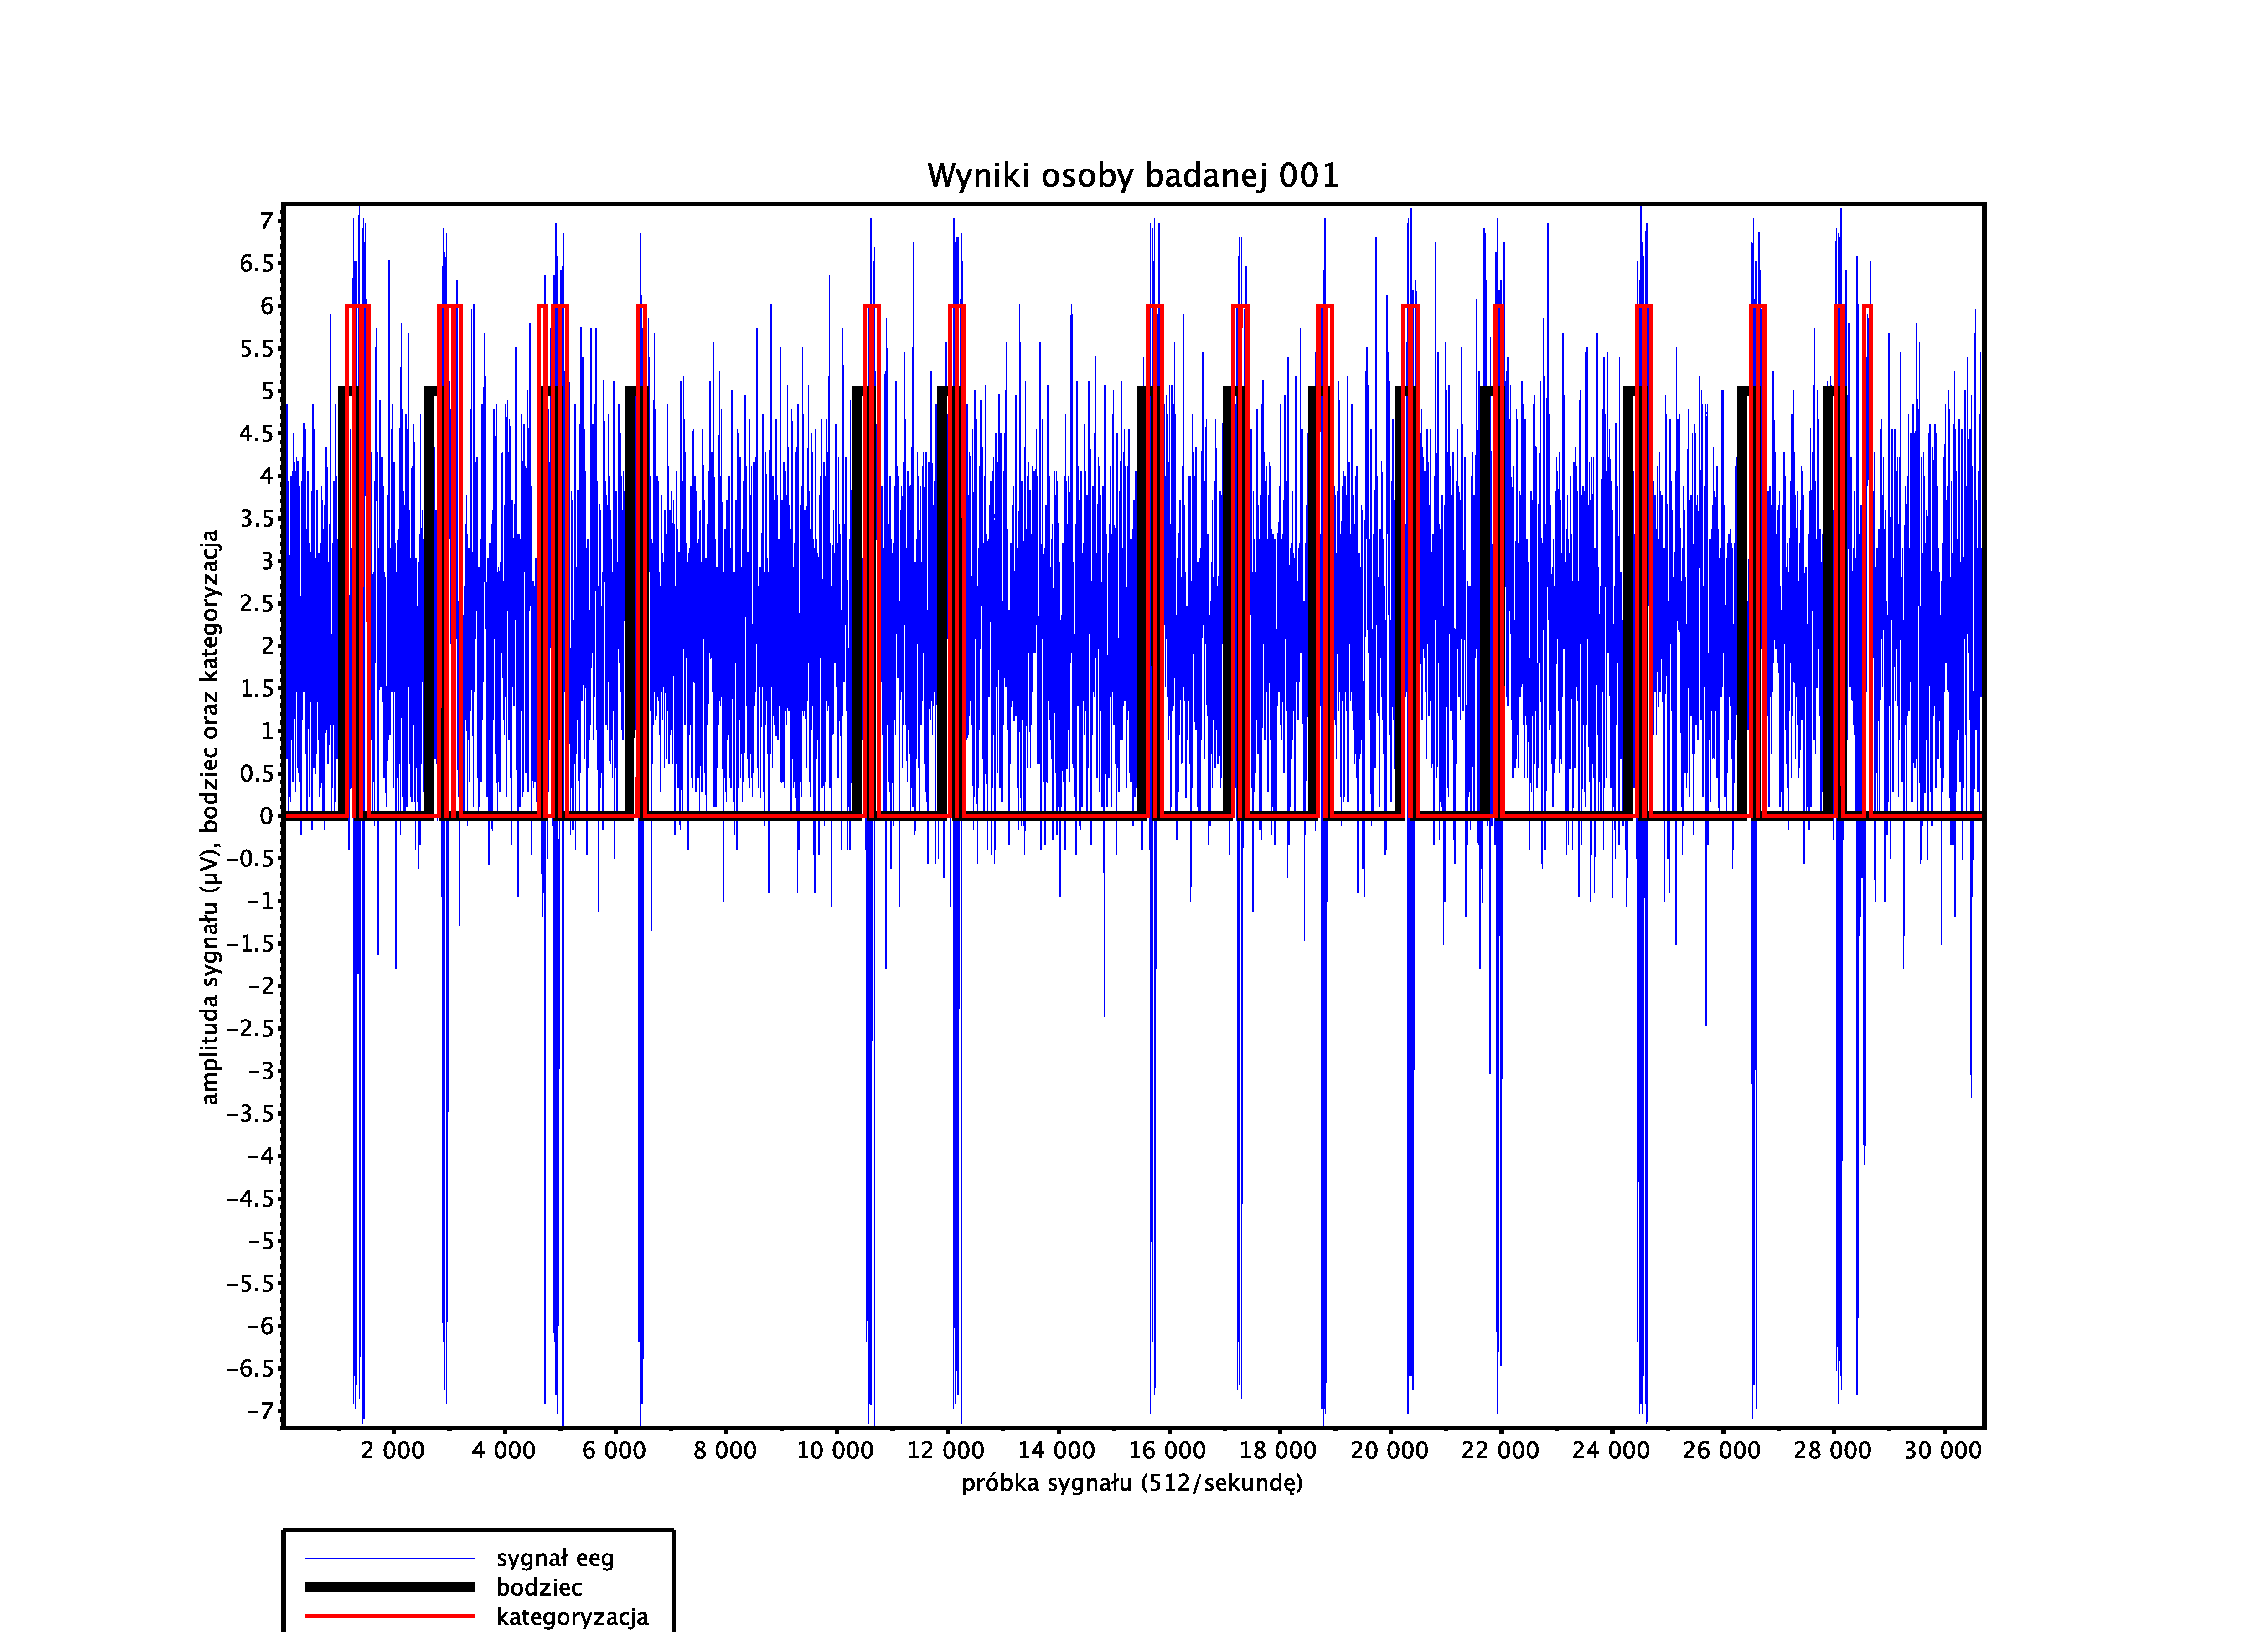
\includegraphics[width=\linewidth+10cm]{../plotting_data/scilab_eeg_01_sub_001.pdf}
            \caption{Dane dla osoby badanej 001}
        \end{sidewaysfigure}
        \begin{sidewaysfigure}[p]
            \hspace*{-4.5cm} 
            \vspace*{1.5cm} 
            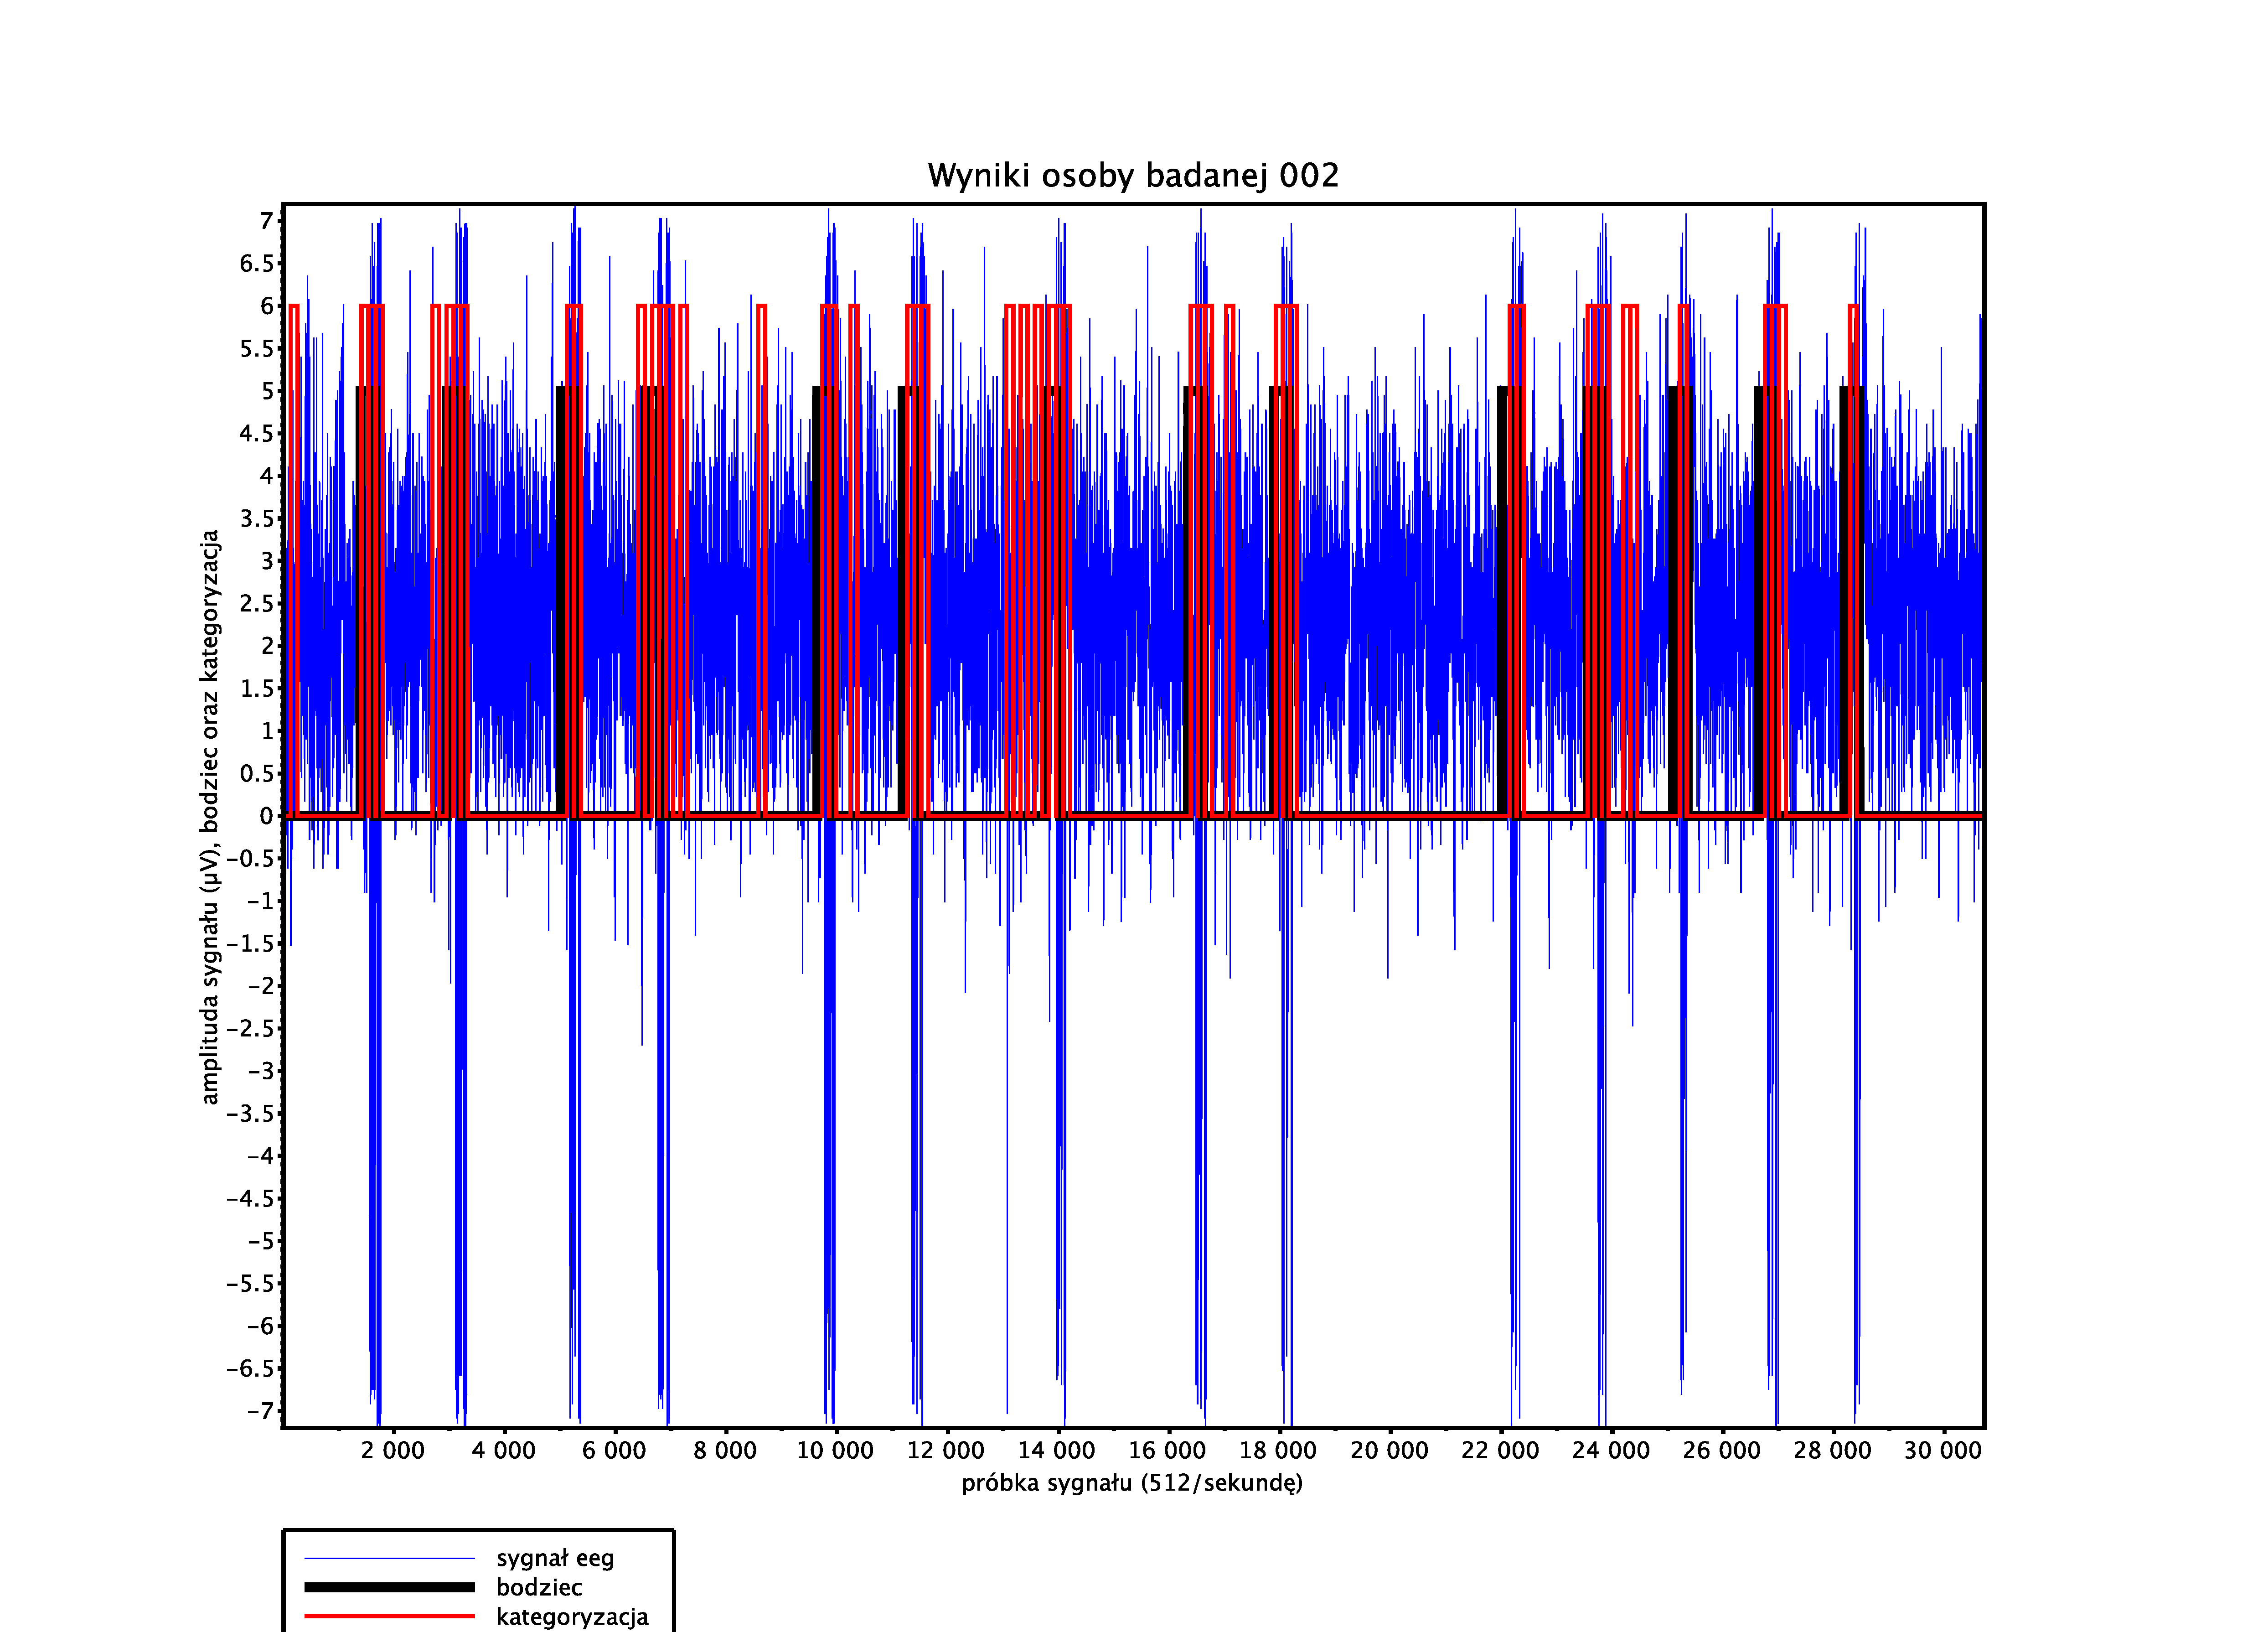
\includegraphics[width=\linewidth+10cm]{../plotting_data/scilab_eeg_01_sub_002.pdf}
            \caption{Dane dla osoby badanej 002}
        \end{sidewaysfigure}
        \begin{sidewaysfigure}[p]
            \hspace*{-4.5cm} 
            \vspace*{1.5cm} 
            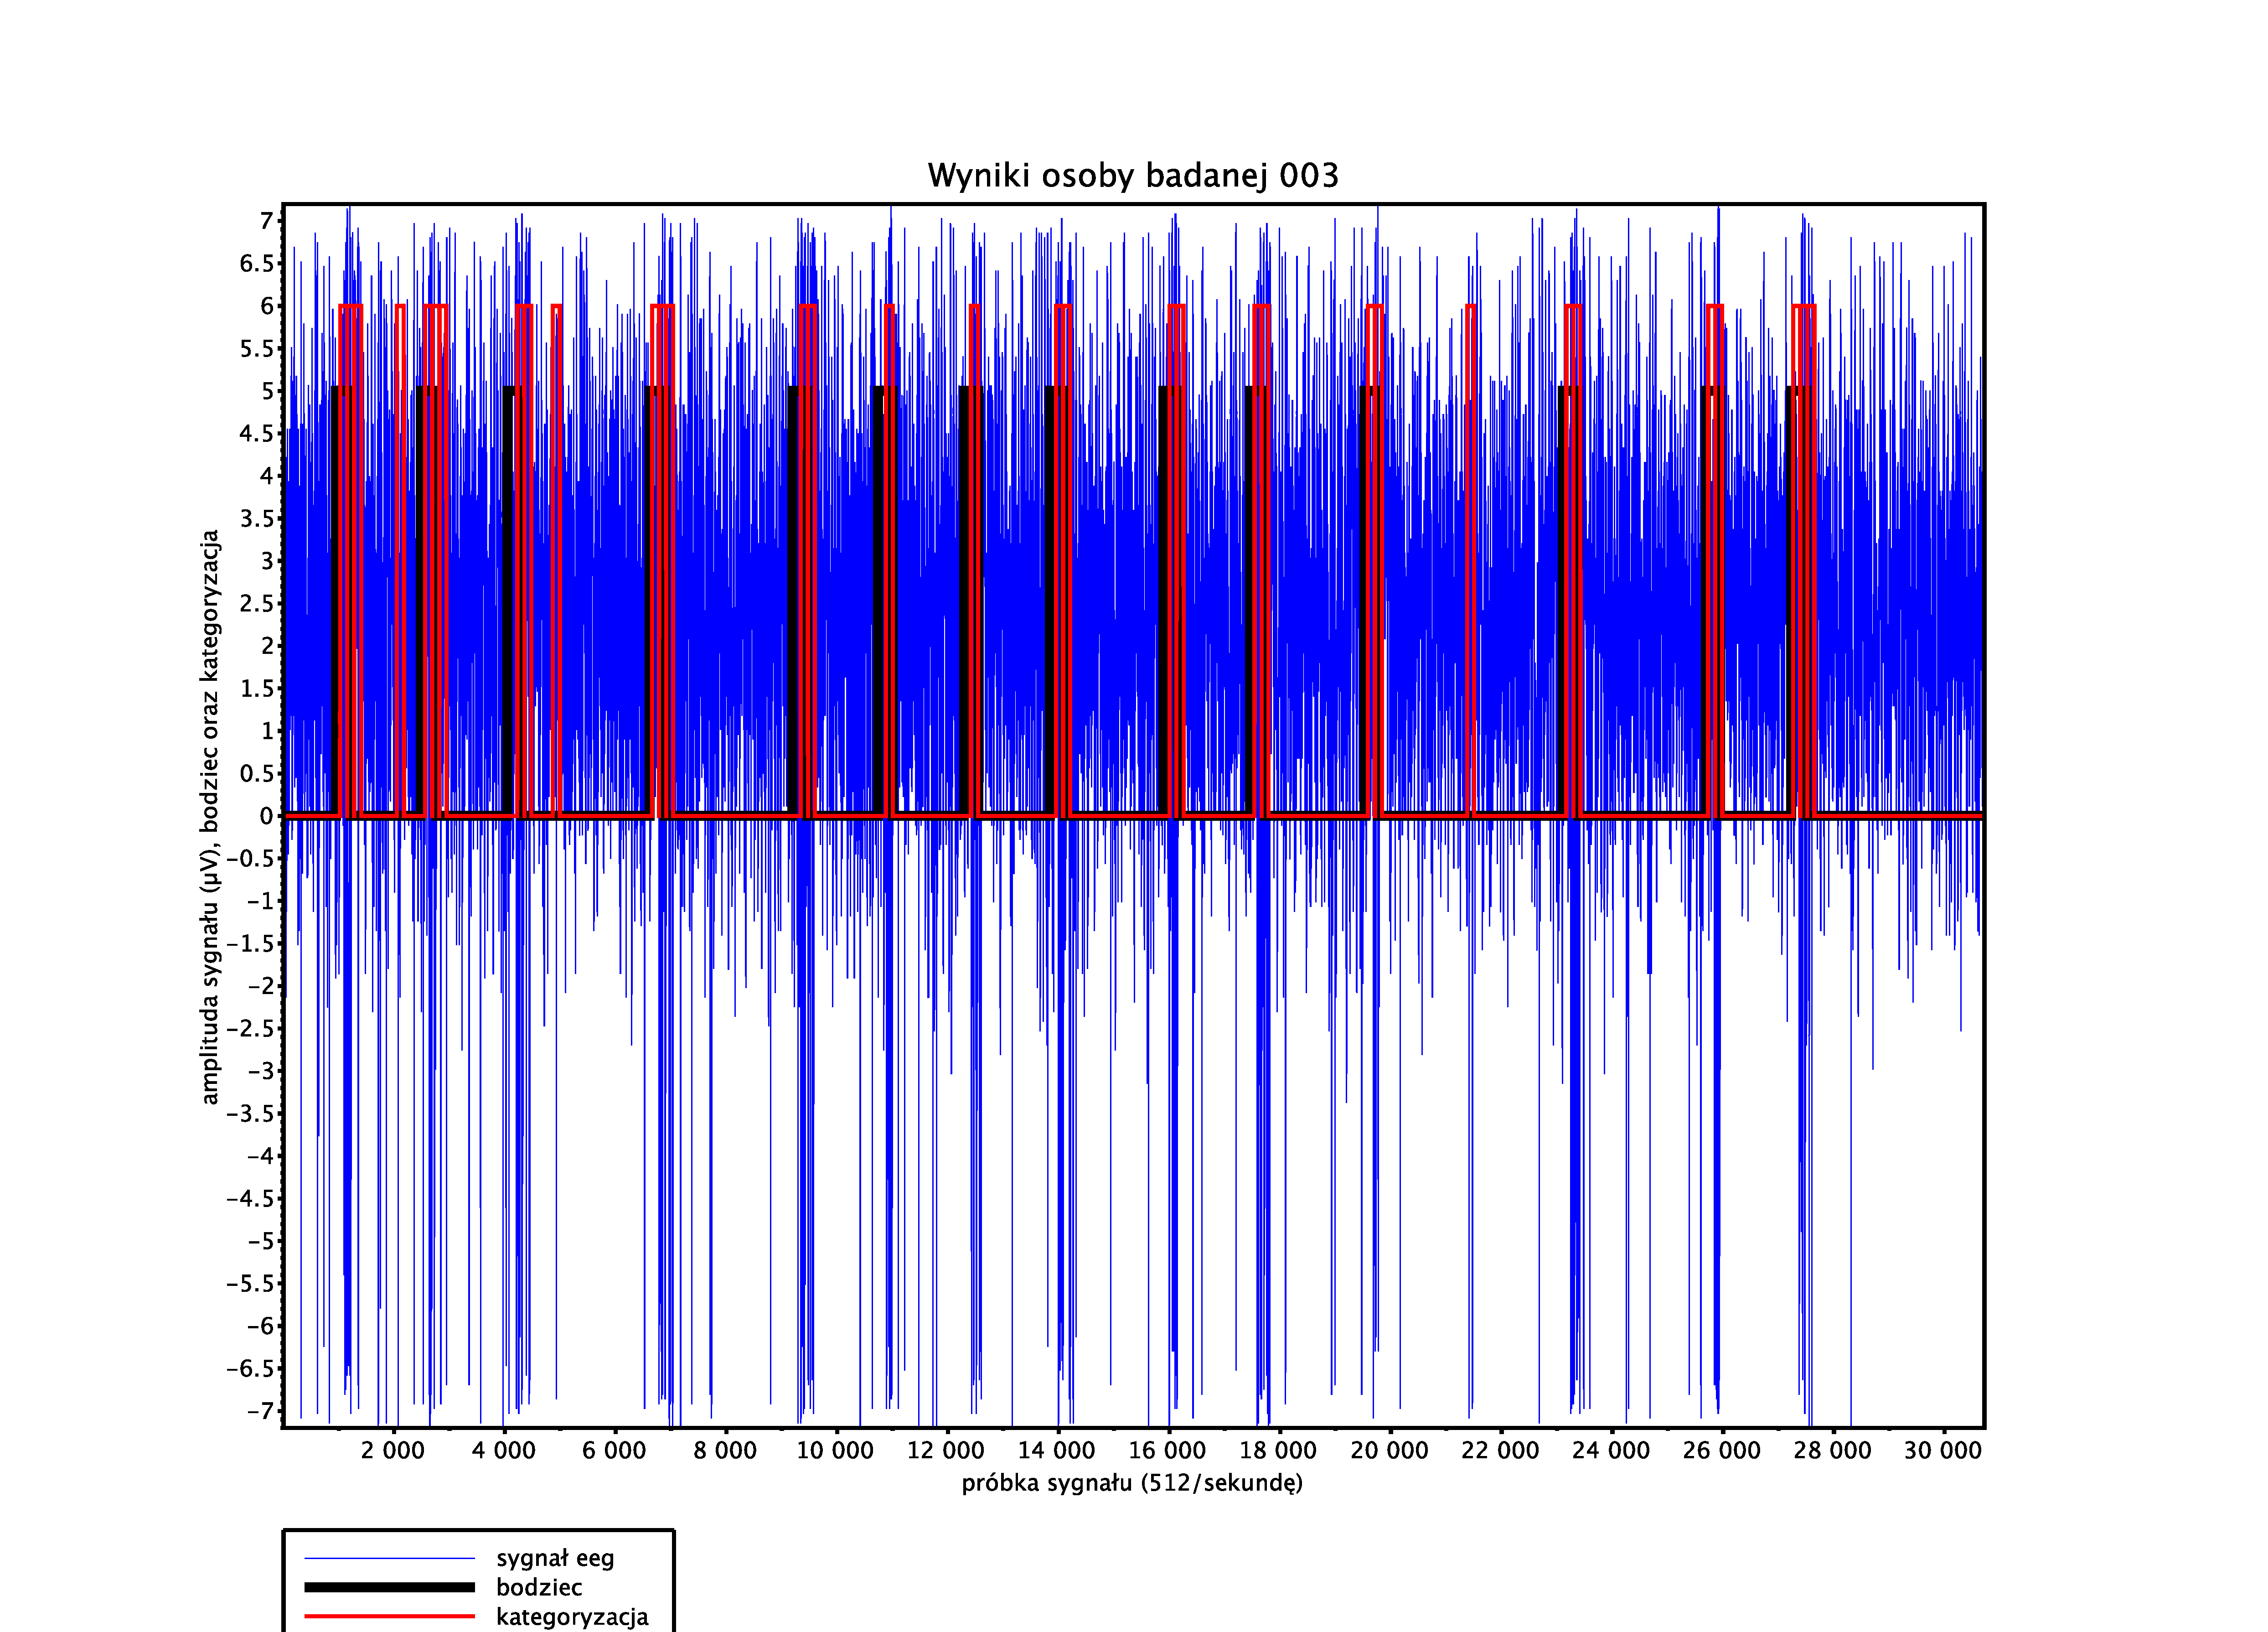
\includegraphics[width=\linewidth+10cm]{../plotting_data/scilab_eeg_01_sub_003.pdf}
            \caption{Dane dla osoby badanej 003}
        \end{sidewaysfigure}
    % % %

%     \newpage
%     \section*{Dodatek C: Podział pracy w grupie}
%         Magdalena Jóźwiakowska::
%         \begin{itemize}
%             \item 
%         \end{itemize}
%         Mikołaj Buchwald:
%         \begin{itemize}
%             \item 
%         \end{itemize}

    % % %

    % \bibliography{bib_eeg_blink_ann}{}
    % \bibliographystyle{plain}

\end{document}
